\documentclass[12pt]{article}
\usepackage{graphicx}
\usepackage{listings}
\usepackage{amsmath}
\usepackage{amssymb}
\usepackage[utf8]{inputenc}
\usepackage[T2A]{fontenc}
\usepackage[russian, english]{babel}
\usepackage[margin=1.5cm,portrait,a4paper]{geometry}
\definecolor{mygreen}{rgb}{0,0.6,0}
\definecolor{mygray}{rgb}{0.5,0.5,0.5}
\definecolor{mymauve}{rgb}{0.58,0,0.82}

\lstset{
    backgroundcolor=\color{white},   % choose the background color
    basicstyle=\footnotesize,        % size of fonts used for the code
    breaklines=true,                 % automatic line breaking only at whitespace
    captionpos=b,                    % sets the caption-position to bottom
    commentstyle=\color{mygreen},    % comment style
    escapeinside={\%*}{*)},          % if you want to add LaTeX within your code
    keywordstyle=\color{blue},       % keyword style
stringstyle=\color{mymauve},     % string literal style
  literate={а}{{\selectfont\char224}}1
           {б}{{\selectfont\char225}}1
           {в}{{\selectfont\char226}}1
           {г}{{\selectfont\char227}}1
           {д}{{\selectfont\char228}}1
           {е}{{\selectfont\char229}}1
           {ё}{{\"e}}1
           {ж}{{\selectfont\char230}}1
           {з}{{\selectfont\char231}}1
           {и}{{\selectfont\char232}}1
           {й}{{\selectfont\char233}}1
           {к}{{\selectfont\char234}}1
           {л}{{\selectfont\char235}}1
           {м}{{\selectfont\char236}}1
           {н}{{\selectfont\char237}}1
           {о}{{\selectfont\char238}}1
           {п}{{\selectfont\char239}}1
           {р}{{\selectfont\char240}}1
           {с}{{\selectfont\char241}}1
           {т}{{\selectfont\char242}}1
           {у}{{\selectfont\char243}}1
           {ф}{{\selectfont\char244}}1
           {х}{{\selectfont\char245}}1
           {ц}{{\selectfont\char246}}1
           {ч}{{\selectfont\char247}}1
           {ш}{{\selectfont\char248}}1
           {щ}{{\selectfont\char249}}1
           {ъ}{{\selectfont\char250}}1
           {ы}{{\selectfont\char251}}1
           {ь}{{\selectfont\char252}}1
           {э}{{\selectfont\char253}}1
           {ю}{{\selectfont\char254}}1
           {я}{{\selectfont\char255}}1
           {А}{{\selectfont\char192}}1
           {Б}{{\selectfont\char193}}1
           {В}{{\selectfont\char194}}1
           {Г}{{\selectfont\char195}}1
           {Д}{{\selectfont\char196}}1
           {Е}{{\selectfont\char197}}1
           {Ё}{{\"E}}1
           {Ж}{{\selectfont\char198}}1
           {З}{{\selectfont\char199}}1
           {И}{{\selectfont\char200}}1
           {Й}{{\selectfont\char201}}1
           {К}{{\selectfont\char202}}1
           {Л}{{\selectfont\char203}}1
           {М}{{\selectfont\char204}}1
           {Н}{{\selectfont\char205}}1
           {О}{{\selectfont\char206}}1
           {П}{{\selectfont\char207}}1
           {Р}{{\selectfont\char208}}1
           {С}{{\selectfont\char209}}1
           {Т}{{\selectfont\char210}}1
           {У}{{\selectfont\char211}}1
           {Ф}{{\selectfont\char212}}1
           {Х}{{\selectfont\char213}}1
           {Ц}{{\selectfont\char214}}1
           {Ч}{{\selectfont\char215}}1
           {Ш}{{\selectfont\char216}}1
           {Щ}{{\selectfont\char217}}1
           {Ъ}{{\selectfont\char218}}1
           {Ы}{{\selectfont\char219}}1
           {Ь}{{\selectfont\char220}}1
           {Э}{{\selectfont\char221}}1
           {Ю}{{\selectfont\char222}}1
           {Я}{{\selectfont\char223}}1
}
\begin{document}
\begin{titlepage}
    \begin{center}
        \vspace*{8cm}
 
        \textbf{Отчет о проделанной работе (Лабораторная работа 4, Вариант 2)}
 
        \vspace{0.5cm}
            Теория вероятностей и математическая статистика
             
        \vspace{1.5cm}
 
        \textbf{Михаил Басанец, Ян Кордияко}
 
        \vfill
             
             
        \vspace{0.8cm}
      
        Белорусский Государственный Университет \\
        Факультет Прикладной Математики и Информатики\\
        2020
             
    \end{center}
\end{titlepage}

\section{Условия}

Рассматривается выборка объемом n = 100. Необходимо 
проверить с помощью критерия хи-квадрат гипотезы $\Pi(1), \  Bi(4, 0.5)$.
\section{Используемые формулы}
\begin{equation}
    \label{eq:1}
    P_{\text{Пуассона}}(k) = \frac{\lambda^k}{k!}e^{-\lambda} \text{ -- функция вероятности р. Пуассона,}
\end{equation}
\begin{equation}
    \label{eq:2}
    P_{\text{биномиальное}}(k) = {{n}\choose{k}}p^k(1 - p)^{n - k} \text{ -- функция вероятности биномиального р.,}
\end{equation}
\begin{equation}
    \label{eq:3}
    \widetilde{\chi^2_n} = n\sum_{j=1}^n\frac{(q_j - p_j(\widetilde{\theta}))^2}{p_j(\widetilde{\theta})} \text{ -- статистика хи-квадрат.}
\end{equation}
\section{Ход работы}
Сначала нарисуем гистограммы гипотетических и выборочного распределений:

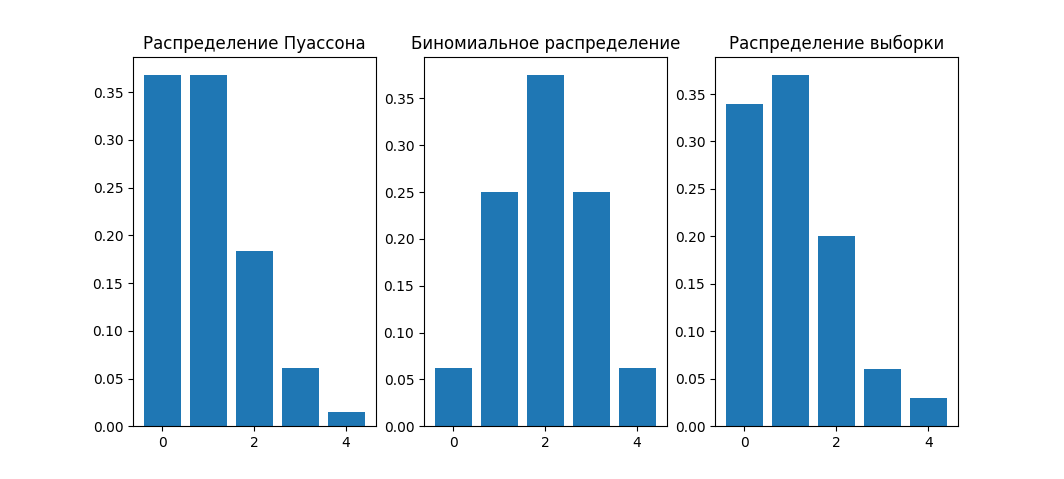
\includegraphics[scale=0.7]{hist}

Как мы можем наблюдать на гистограммах, распределение выборки довольно
сильно напоминает распределение Пуассона, в то время как оно значительно
отличается от биномиального распределения. Проверим наши наблюдения с помощью
критерия хи-квадрат.

Для начала разделим выборку на интервалы. В качестве интервалов возьмём:
$$[0, 1), [1, 2), [2, 3), [3, 4), [4, 5).$$ 
Так как количество элементов, попавших в 
последний интервал менее 5, то объединим его с предыдущим. 
Таким образом, получим
$l = 4$ интервала: $$\Delta_1 = [0, 1), \Delta_2 = [1, 2), \Delta_3 = [2, 3), \Delta_4 = [3, 5).$$

Теперь подсчитаем эмпирические вероятности попадания в соответствующие интервалы:
$$q_1 = 0.34, q_2 = 0.37, q_3 = 0.2, q_4 = 0.09.$$

Затем для подсчитаем теоритические вероятности 
попадания в соответствующие интервалы для распределения Пуассона
с помощью \eqref{eq:1}:
$$p_1 = 0.36787944117144233,\  p_2 = 0.36787944117144233,$$$$ p_3 = 0.18393972058572114, 
\  p_4 = 0.07664155024405049.$$

Теперь подсчитаем статистику хи-квадрат \eqref{eq:3}:
$$\widetilde{\chi^2_n} = 0.5855658625776508$$

Распределение Пуассона имеет $k = 1$ степень свободы. Также
возьмём уровень значимости $\alpha = 0.05$. Следовательно,
находим в соответствующей таблице пороговое значение статистики хи-квадрат
$$C_{0.05} = \chi^2_{0.05,\  l - k - 1} = 5.991.$$

Очевидно, что $\widetilde{\chi^2_n} < C_{0.05}$, следовательно данная гипотеза принимается.

Теперь проверим критерий хи-квадрат для биномиального распределения.
Сначала подсчитаем теоритические вероятности 
попадания в соответствующие интервалы для этого распределения
с помощью \eqref{eq:2}:
$$p_1 = 0.0625,\  p_2 = 0.25000000000000006,$$$$ p_3 = 0.3750000000000001, 
\  p_4 = 0.31250000000000006.$$

Теперь подсчитаем статистику хи-квадрат \eqref{eq:3}:
$$\widetilde{\chi^2_n} = 152.97866666666673$$

Биномиальное распределение имеет $k = 2$ степени свободы. Также
возьмём уровень значимости $\alpha = 0.05$. Следовательно,
находим в соответствующей таблице пороговое значение статистики хи-квадрат
$$C_{0.05} = \chi^2_{0.05,\  l - k - 1} = 3.841.$$

Очевидно, что $\widetilde{\chi^2_n} > C_{0.05}$, причём понятно, что при любом другом
адекватном уровне значимости $\alpha$ неравенство сохранит знак. Следовательно,
данная гипотеза отвергается.
\section{Выводы}

Критерий проверки гипотезы Пирсона подтвердил наши наблюдения, основанные на
сравнительных гистограмах. Распределение выборки оказалось близким к распределению
Пуассона, но совсем не похожим на биномиальное распределение.
\section{Исходный код программы}
\lstinputlisting[language=Python]{main.py}
\end{document}